\documentclass{article}
\usepackage[utf8]{inputenc}
\usepackage[round]{natbib}
\usepackage[colorlinks=true, citecolor=blue]{hyperref}
\usepackage[T1]{fontenc}
\usepackage[french,english]{babel}
\usepackage{textcomp}
\usepackage{verbatim}
\usepackage{amsmath}
\usepackage{amssymb}
% \usepackage{booktabs}
\usepackage{threeparttable}
% \usepackage{hyperref}
\usepackage{lscape}
\usepackage{pifont}
\newcommand{\cmark}{\ding{51}}
\newcommand{\xmark}{\ding{55}}
\usepackage{chngpage}
\usepackage{array}
\usepackage{multirow}
\usepackage{graphicx}
\usepackage[export]{adjustbox}
\usepackage{float}
\usepackage{geometry}
\usepackage{booktabs,multirow,makecell}
\usepackage{tabularx}
\usepackage{tikz}
\usetikzlibrary{calc,positioning,fit}
\usepackage{xcolor}
\geometry{hmargin=3.5cm,vmargin=2.5cm}
\usepackage[justification=centering]{caption}
\title{Role of forest biomass in the Finnish decarbonization\footnote{PhD student at University of Pisa}\footnote{mail. m.bordenave@student.unisi.it}\footnote{\url{https://orcid.org/0000-0002-5571-5877}}}
\author{Matthieu Bordenave}
\date{\today}

\begin{document}

\maketitle{}

\begin{abstract}
Woody biomass plays a central role in many deep decarbonization narratives for Finland, where high forest cover and an established forest industry make lignocellulosic resources a key option for heat, power, fuels, and non-energy demand. At the same time, the contribution of forest biomass is deeply uncertain because it depends on biodiversity protection rules, carbon sink objectives, and exposure to forest physical risks such as storms, wildfires, and pests, which can generate both availability shocks and market price disruptions. This article develops a preliminary, first-stage modelling framework to explore these tensions using EnergyScope TD, a whole-energy system optimisation model based on a reduced set of representative typical days. Building on the EnergyScope Multi-Cells dataset for Finland (hourly reference year 2017, UTC), the paper documents the end-use demand mapping in energy services, the time-series inputs used for typical-day selection, and a Finland-specific calibration workflow. For biomass, the first stage reproduces the modelling base proposed by Colla et al. for lignocellulosic supply representation, conversion pathways, costs, and import segmentation, in order to ensure comparability and to focus the analysis on allocation across competing end-uses under a binding greenhouse-gas constraint. The second stage, introduced as a scenario design, translates alternative policy and risk narratives into transparent shifts of biomass supply-curve availability and marginal costs. Simulation results are currently under production; this version therefore emphasises the modelling architecture, calibration choices, and scenario logic that will support a systematic assessment of the role and limits of forest biomass in Finnish decarbonization pathways.
\end{abstract}


\begin{displaymath}
\\
\end{displaymath}

\textbf{Keywords:} 
\begin{center}
\begin{tabular}{p{5cm}}
\\
\end{tabular}
\end{center}

\textbf{JEL classification codes:} 

\newpage

\section*{Introduction}


Finland's pathway to deep decarbonisation sits at the intersection of three system constraints: electrifying end uses at scale, integrating high shares of variable renewables with adequate storage and flexibility, and managing a uniquely large forest biomass resource under increasing scrutiny about carbon accounting and biodiversity impacts. In this context, energy planning tools are not only asked to identify least-cost technology mixes, but also to make explicit cross-sector trade-offs between electricity, heat and mobility, and the role of renewable fuels and carbon capture options where direct electrification is difficult.

This paper develops a first national application of EnergyScope TD to the Finnish energy system. EnergyScope TD is an open-source, linear programming, whole-energy system model that optimises both investment and operation for a target year, with an hourly representation through a typical-days reduction. This makes it suitable for scenarios with high penetration of intermittent renewables and storage \citep{limpens_energyscope_2019,limpens_energyscope_2024}. By construction, it provides an open source and computationally efficient framework for exploring alternative transition constraints.

Methodologically, the first contribution is to build and document a Finland-specific dataset and calibration for a 2050 snapshot analysis, consistent with EnergyScope TD requirements (end-use demands, technology portfolio, resource potentials, and time series for key variables). The second contribution is model verification through historical reproduction. Following the approach used for Switzerland and Belgium, we constrain the model with observed end-use demands and technology shares for a past reference year and compare model outputs to reported energy balances and emissions, as a practical test of the model's ability to represent a national system \citep{moret_characterization_2017,thiran_exploring_2025,limpens_generating_2021}.

The core research question is: what will be the role of forest biomass in the Finnish energy transition by 2050, and how does this role change when carbon capture and storage (CCS) technologies are available? This question is particularly important because many whole-energy system models wrongly treat biomass as carbon neutral, which can strongly shape optimal outcomes. Building on the scenario-analysis tradition in EnergyScope applications, we examine contrasting biomass potential assumptions, including conservative and biodiversity-protective availability constraints, and test how these constraints interact with electrification, hydrogen, and renewable fuel pathways.

\begin{enumerate}
  \item \textbf{Model credibility:} To what extent can a constrained EnergyScope TD setup reproduce Finland's observed energy balances and combustion emissions for a past reference year (within acceptable error margins), providing confidence for forward-looking scenario analysis?
  \item \textbf{Biomass role:} Under a 2050 decarbonisation target, how much forest biomass is allocated across heat, power, industry and transport, and what are the implied system costs and technology choices under alternative biomass availability constraints?
  \item \textbf{CCS interaction:} How do CCS and BECCS options reshape the optimal use of biomass (for example, as a scarce fuel for hard-to-electrify sectors versus a feedstock for negative emissions), and what trade-offs emerge with other flexibility options and renewable fuels?
\end{enumerate}


\section{Model description: EnergyScope TD}

\subsection{Positioning in the energy system modelling literature}
EnergyScope TD is a whole-energy system optimisation model designed for scenario analysis of regional or national energy transitions with high temporal resolution while keeping computational times compatible with extensive sensitivity and uncertainty analyses. In contrast with power-only optimization tools, EnergyScope TD represents power, heating, and mobility (and, depending on the implementation, non-energy demand, e.g amonium) within a single, demand-driven energy balance framework. A central design choice is the use of a limited set of representative "typical days" (TDs) to approximate intra-annual variability, combined with a reconstruction mechanism that preserves inter-day storage dynamics.

This modeling choice responds to a broader pattern identified in the deep decarbonisation literature. Based on a review of European decarbonisation scenario studies, \citet{borasio_deep_2022} highlight both the diversity of modelling practices and a recurrent trade-off between scope and tractability: many studies rely either on top-down approaches or on tools primarily centered on the power sector, while fewer frameworks represent sector coupling across power, heat and mobility in a consistent optimisation setting. This motivates the use of whole-energy system models that can capture cross-sectoral substitutions and flexibility needs while remaining sufficiently lightweight for systematic scenario exploration.

A key motivation for EnergyScope TD is therefore that combining (i) multi-sector coverage, (ii) open-source availability, (iii) endogenous system design and operation, and (iv) short runtimes is uncommon in large-scale energy planning practice. Table~\ref{tab:model-comparison} summarises this positioning using the comparative criteria reported in \citet{limpens_energyscope_2019}.

\begin{table}[t]
  \centering
  \renewcommand{\arraystretch}{1.15}
  \begin{tabularx}{\linewidth}{lcccc}
    \toprule
    \textbf{Model} & \textbf{Multi-sector} & \textbf{Open-source} & \textbf{Optimisation} & \textbf{Comp. time} \\
    \midrule
    Calliope        & \cmark & \cmark & \cmark & mins \\
    COMPOSE         & \cmark & \xmark & \cmark & - \\
    DESSTinEE       & \cmark & \cmark & \xmark & s \\
    DIETER          & \xmark & \cmark & \cmark & mins \\
    EnergyPLAN      & \cmark & \xmark & operation only  & s \\
    MARKAL/TIMES    & \cmark & \xmark & investment only & 5-35 min \\
    oemof           & \cmark & \cmark & \cmark & mins \\
    OSeMOSYS        & \cmark & \cmark & \cmark & mins \\
    PyPSA           & \cmark & \cmark & \cmark & mins \\
    STREAM          & \cmark & \xmark & \xmark & - \\
    Switch          & \xmark & \cmark & \cmark & 10-60 min \\
    URBS            & \xmark & \cmark & \cmark & 20 min \\
    \addlinespace
    \textbf{EnergyScope TD} & \textbf{\cmark} & \textbf{\cmark} & \textbf{\cmark} & \textbf{$\sim$1 min} \\
    \bottomrule
  \end{tabularx}
  \caption{Indicative comparison of large-scale energy planning models along four criteria commonly used in the energy optimisation model literature: multi-sector scope, open-source status, optimisation of both design and operation, and order-of-magnitude runtime per scenario. Adapted from the comparison reported in \citet{limpens_energyscope_2019}.}
  \label{tab:model-comparison}
\end{table}

EnergyScope TD is part of a broader open modeling family. Historically, EnergyScope was first developed with coarser temporal aggregation and later extended toward hourly resolution with TDs and seasonality in EnergyScope TD, and further toward multi-regional representations in EnergyScope Multi-Cell \citep{hernandez_energyscope_2021,thiran_exploring_2025,borasio_deep_2022}.

A common critique of EnergyScope TD, also emphasised in reviews of deep decarbonisation modelling, concerns spatial representation. Single-node national models may abstract from intra-country congestion, regional renewable heterogeneity, and the location of flexible demand, which can matter when electrification and variable renewables expand rapidly \citep{borasio_deep_2022,limpens_energyscope_2024}. In the Finnish case, however, a first-order single-region representation is arguably more defensible than in countries with multiple dense load centers, because population, most energy demand, and the bulk of industrial activity are concentrated in the South, where the main transmission backbone and urban heat loads are also located. This motivates using EnergyScope TD for the purpose of our research interests. 


In climate-mitigation narratives, biomass is often framed as a renewable and flexible resource, yet estimates of its future contribution remain highly uncertain because they depend on the constraint set adopted, including sustainability rules, technical feasibility, land and biodiversity limits, and economic conditions. Under sustainability-oriented assumptions, \citet{beringer_bioenergy_2011} report a wide global range for bioenergy in 2050 (126--216~EJ), broadly consistent with other assessments that apply different constraint sets and therefore obtain markedly different potentials \citep{haberl_global_2010,schueler_global_2013,searle_reassessment_2015,strapasson_global_2017,iea_bioenergy_2023}. At present, biomass already constitutes a substantial fraction of renewable energy supply and is used predominantly for heat \citep{iea_key_2020,iea_bioenergy_2023}. Looking forward, deep decarbonisation implies defossilising multiple sectors simultaneously, which can increase competition for lignocellulosic resources as they are called upon to provide not only heat and power but also transport fuels and carbon-based feedstocks for industry and chemicals \citep{wwf_energy_2011,daioglou_competing_2015}. Hence, the key transition question is not only \emph{how much} biomass can be mobilised, but also \emph{where} it should be allocated across final needs once economy-wide greenhouse-gas constraints bind \citep{colla_optimal_2022}.

A central theme in the biomass literature is that pathway comparisons should be made at the level of delivered services rather than solely at the level of produced fuels. Substitution logics distinguish fuel-level substitution from energy-service substitution, where the avoided emissions depend jointly on conversion efficiencies and on the demand-side technologies that ultimately use the energy carrier \citep{wahlund_increasing_2004}. In this view, conversion losses in biofuel production may be compensated if the carrier enables substantially more efficient end-use devices \citep{steubing_heat_2012}. This mechanism becomes visible in whole-system optimisation: \citet{codina_girones_optimal_2017} compare woody-biomass conversion routes inside a national energy-system optimisation and show that biofuel pathways can outperform direct biomass combustion in avoided \ce{CO2} only when accompanied by a broader shift toward efficient end-use options (for instance heat pumps or battery electric vehicles).


Taken together, these insights motivate the use of whole-energy system optimisation frameworks that decide endogenously both (i) how much biomass to use and (ii) how to distribute it across heat, electricity, mobility fuels, and material uses, conditional on the rest of the energy system and on emissions constraints. In that spirit, \citet{colla_optimal_2022} implement a detailed lignocellulosic biomass representation in EnergyScope TD and analyse how optimal allocations shift as GHG constraints tighten, providing a documented modelling base that can be transferred to new country contexts.



\subsection{Two-step methodology and data flow}
EnergyScope TD is typically implemented as a two-step workflow:
(i) a temporal aggregation step that selects a small set of TDs (and their weights and sequence), and
(ii) a linear programming (LP) optimisation step that determines the least-cost (or otherwise constrained) energy system configuration for a target year under the TD representation \citep{limpens_generating_2021}.

\begin{figure}[h!]
  \centering
  % Replace with your exported figure file (e.g. from Limpens 2019) if you plan to reproduce it
  \includegraphics[width=0.95\linewidth]{steps.png}
  \caption{Schematic overview of the two-step EnergyScope TD workflow: Step 1 selects typical days and reconstructs a year; Step 2 solves the energy system optimisation problem on the reduced time basis. Based on the framework presented in \citet{limpens_energyscope_2019}.}
  \label{fig:workflow}
\end{figure}

\subsection{Step 1: Selecting typical days}
In the EnergyScope framework, Step 1 is dedicated to the selection of a subset of representative days, known as typical days (TDs), to overcome the "curse of dimensionality" and reduce the computational time of the energy system optimisation from over 19 hours to approximately one minute.

\subsubsection{Inputs and preprocessing}
Step 1 starts from hourly time series intended to represent the main drivers of intra-annual variability in supply and demand. In the EnergyScope TD applications discussed by \citet{limpens_generating_2021}, the TD selection is built from a small set of demand and weather series, including electricity demand, heat demand, solar irradiance, and wind (onshore and offshore) profiles (See Table \ref{tab:fi_td_inputs_sources}). The series are normalised and weighted to ensure that the TD set captures the most decision-relevant variability for system design (for instance, by giving more emphasis to electricity and heating profiles when studying flexibility and storage).

% ------------------------------------------------------------------
% Insert this in \subsection{Step 1: Selecting typical days},
% inside \subsubsection{Inputs and preprocessing},
% AFTER your first sentence introducing hourly inputs,
% and BEFORE the \subsubsection{Clustering and representative-day selection}.
% ------------------------------------------------------------------

For Finland, we rely first on the pre-compiled hourly profiles distributed with the EnergyScope Multi-Cells database \cite{thiran_exploring_2025}. All time series are provided on a common historical reference year (2017) to ensure synchronicity across demand drivers and weather-dependent renewable availability. These inputs are used both to construct the typical days and to drive the hourly constraints of the optimisation model.

\begin{table}[t]
\centering
\footnotesize
\caption{Hourly time series used in EnergyScope Multi-Cells for Finland to build typical days (TDs) and to drive the optimisation model \citep{thiran_exploring_2025}. All profiles are synchronous and based on a common reference year (2017, UTC).}
\label{tab:fi_td_inputs_sources}
\begin{tabular}{p{3.1cm}p{5.6cm}p{5.4cm}}
\toprule
\textbf{Series (file column)} & \textbf{Meaning in the model} & \textbf{Main data source and processing} \\
\midrule
ELECTRICITY & Specific electricity hourly share (normalised) & ENTSO-E Transparency load (via OPSD), subtract electric heating and cooling (HRE4-based dispatch), then normalise. \\
HEAT\_LOW\_T\_SH & Space heating hourly share (normalised) & OPSD country temperature from MERRA-2; compute heating-degree-hours with 14$^\circ$C threshold; apply 24h moving average; normalise. \\
SPACE\_COOLING & Space cooling hourly share (normalised) & OPSD country temperature from MERRA-2; compute cooling-degree-hours with 20$^\circ$C threshold; apply 24h moving average; normalise. \\
MOBILITY\_PASSENG. & Passenger mobility hourly share & NHTS-based hourly profile, kept as in EnergyScope TD Belgium. \\
MOBILITY\_FREIGHT & Freight mobility hourly share & In the released dataset this profile is flat over the year (no temporal structure). \\
\midrule
PV & PV capacity factor (GW/GWp) & Renewable.ninja country-aggregated profiles (via OPSD); used for rooftop and utility PV. \\
WIND\_ONSHORE & Onshore wind capacity factor & Renewable.ninja country-aggregated profiles (via OPSD). \\
WIND\_OFFSHORE & Offshore wind capacity factor & Renewable.ninja profiles (via OPSD), with reconstruction or proxy rules for missing historical series. \\
SOLAR & Solar thermal proxy capacity factor & Derived from GHI using OPSD weather data computed from MERRA-2. \\
CSP & CSP thermal output proxy & DNI from PVGIS (via pvlib) and thermal output computed with Oemof thermal; representative plant location. \\
HYDRO\_RIVER & Run-of-river capacity factor & Daily run-of-river generation (JRC-EFAS, completed by ENTSOE-PECD), interpolated to hourly and normalised. \\
HYDRO\_DAM & Hydropower inflow proxy capacity factor & Weekly inflow (JRC-EFAS, completed by ENTSOE-PECD), interpolated to hourly and normalised. \\
TIDAL & Tidal capacity factor & Literature-based tidal profile, rescaled to match an average capacity factor assumption. \\
\bottomrule
\end{tabular}
\end{table}


Demand-side series are expressed as normalised hourly profiles (shares over the year), which makes the typical-day selection focus on temporal patterns rather than absolute annual levels. Weather-dependent renewable series are expressed as capacity factors, preserving intra-day and seasonal variability in PV, wind, and hydro. For Finland, this implies that space heating drives strong winter seasonality, while PV adds a pronounced day-night and summer-winter structure, and wind contributes irregular day-to-day variability.


To document the typical-day construction step, Figures~\ref{fig:fi_td_demand_heatmaps}--\ref{fig:fi_td_duration_curves} display the pre-compiled hourly time series used as inputs in EnergyScope Multi-Cells for Finland (reference year 2017, UTC). Demand drivers are expressed as normalised hourly profiles (shares of annual totals), while renewable availability is expressed as capacity-factor type profiles.

% ------------------------- Demand heatmaps -------------------------
\begin{figure}[h!]
  \centering
  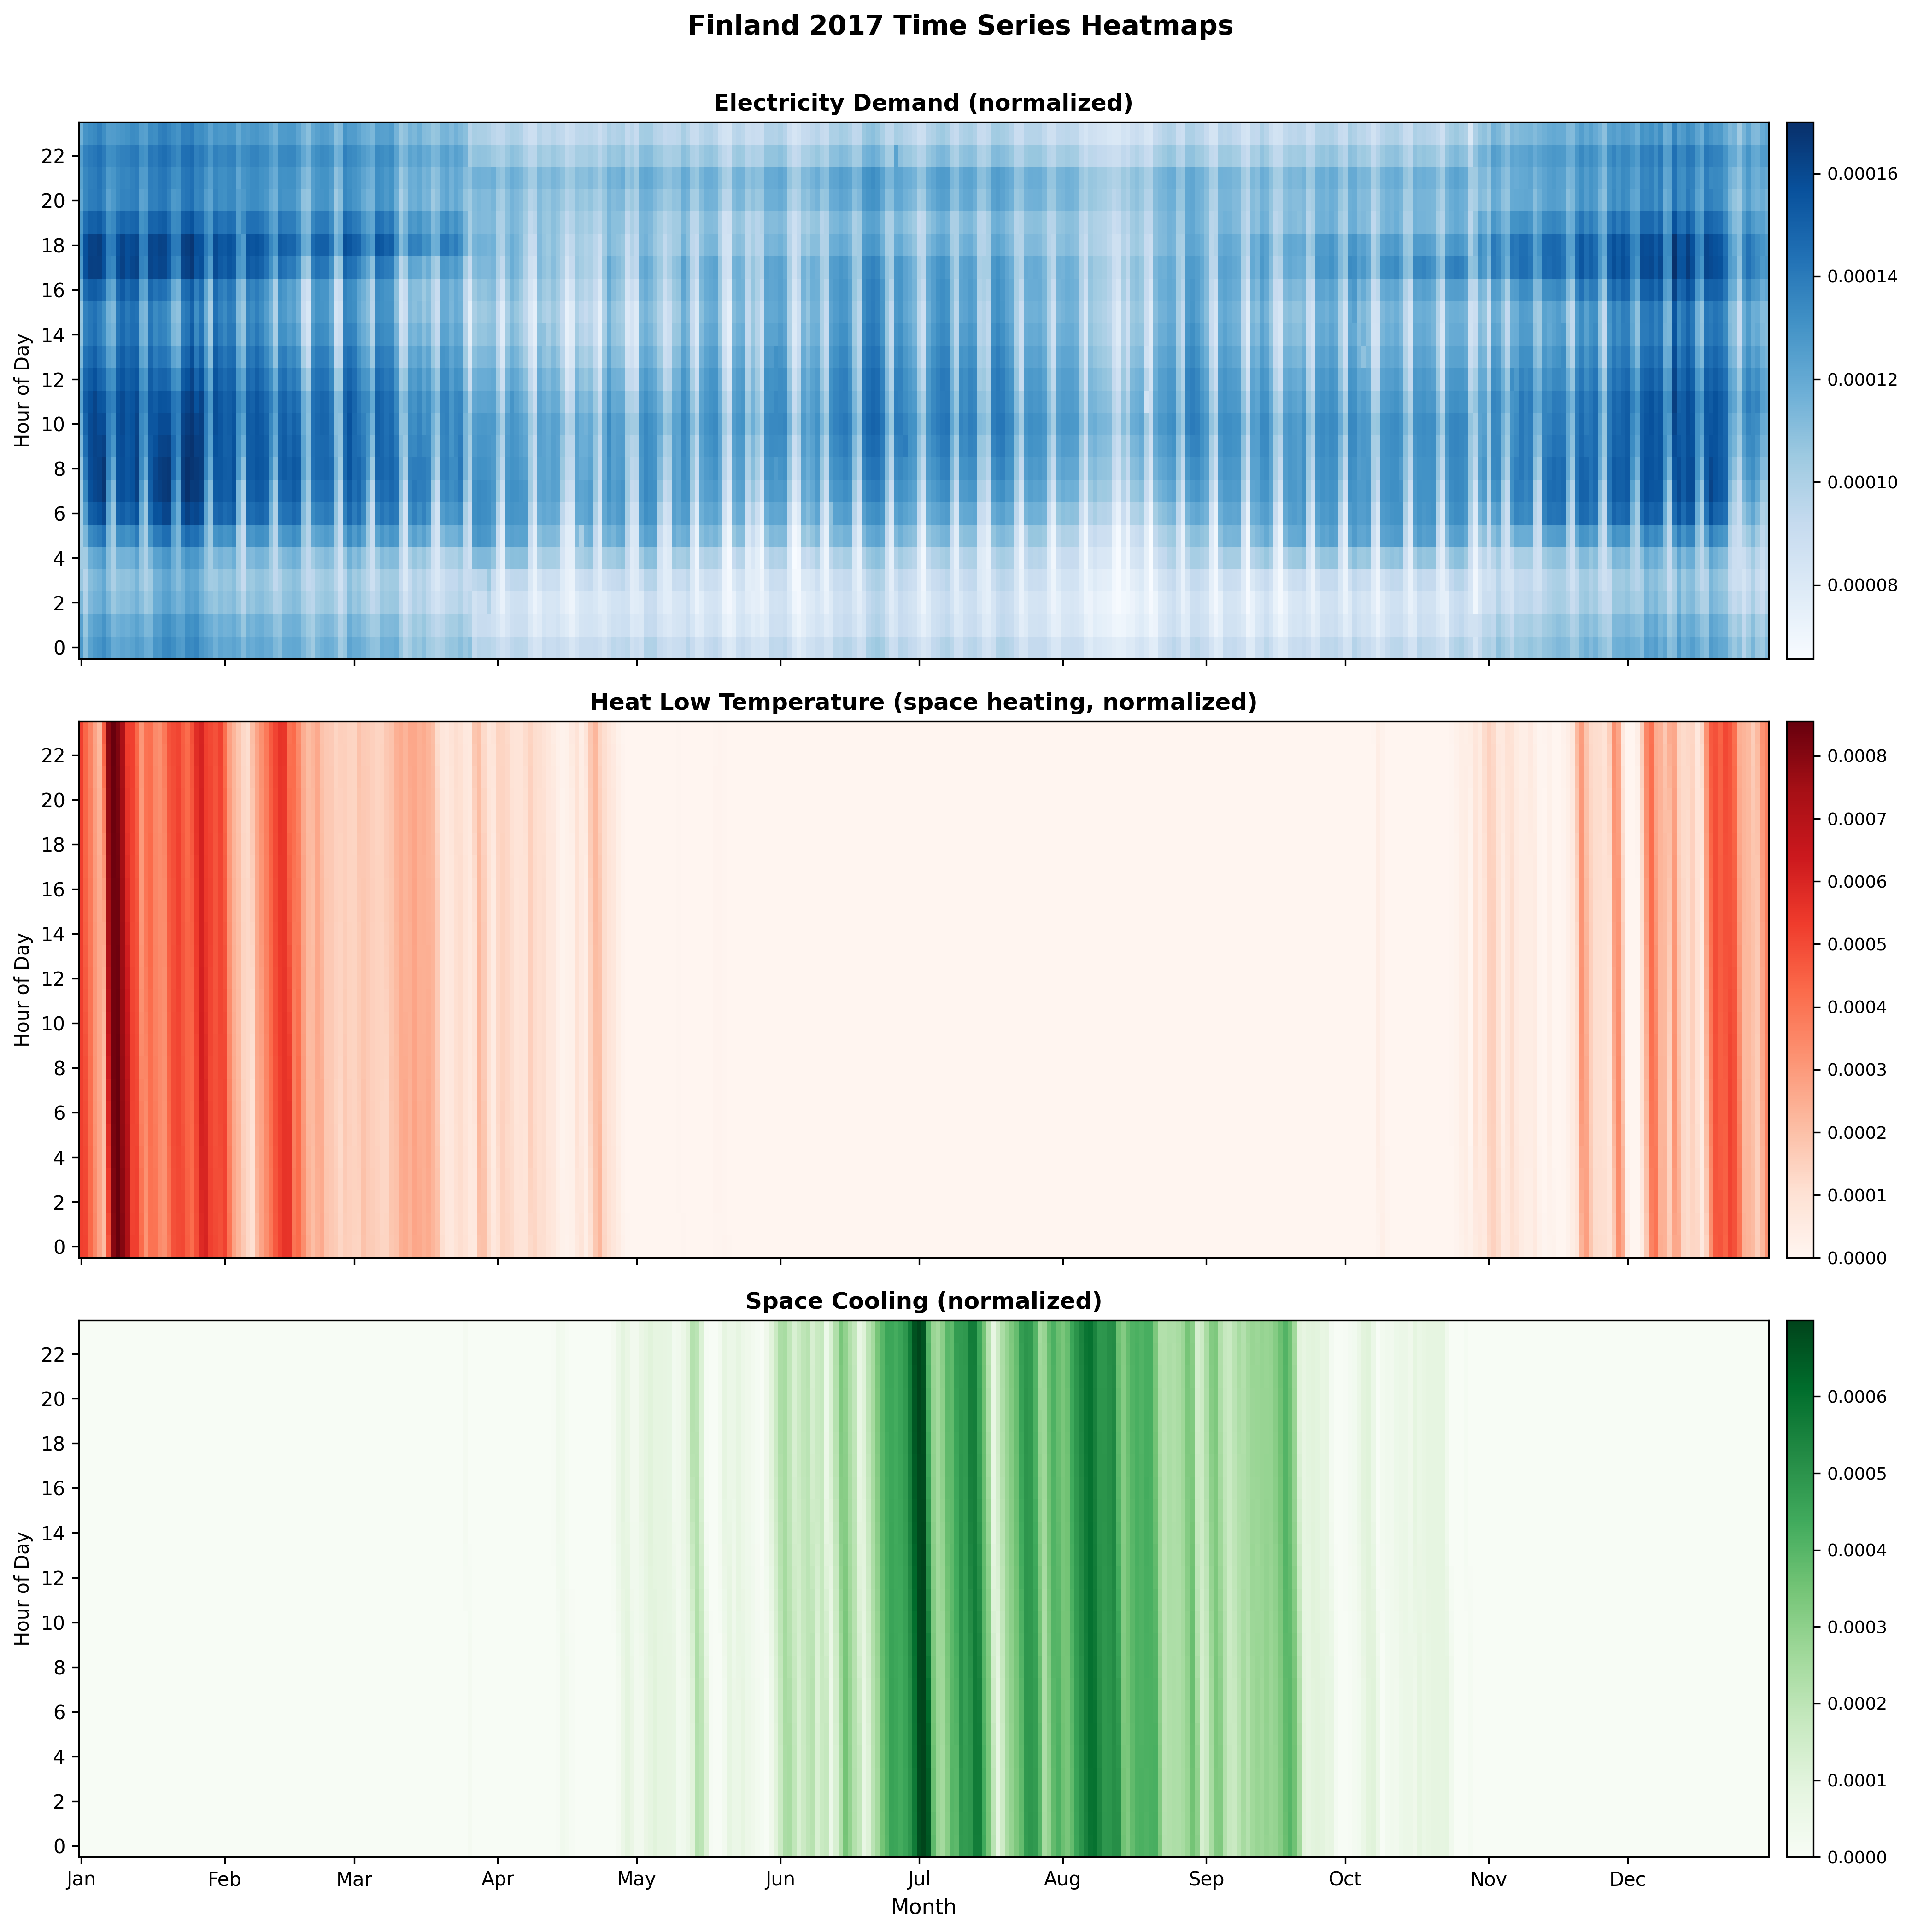
\includegraphics[width=\linewidth]{fi_heatmaps_combined.png}
  \caption{Finland (2017, UTC): demand-driver heatmaps used in the typical-day preprocessing. Each panel shows the distribution of hourly demand over the year (normalised profiles), with months on the x-axis and hour of day on the y-axis.}
  \label{fig:fi_td_demand_heatmaps}
\end{figure}

The electricity profile exhibits both intra-day structure (systematic daily cycles) and a marked seasonal component, with the largest total shares occurring during the cold season even though summer daytime load remains visible. Low-temperature space-heating demand is strongly seasonal, with a pronounced winter concentration and near-zero levels in summer, reflecting its degree-hour construction. Space-cooling appears as a sparse summer phenomenon, indicating that cooling is a minor driver in the Finnish context and contributes limited discriminatory information outside the warmest weeks. Because all demand series are normalised, the colour intensity should be read as the relative allocation of annual demand across hours rather than absolute load levels.


\begin{figure}[H]
  \centering
  
\includegraphics[width=0.78\linewidth]{FI_2017_mobility_passenger_daily_profile.png}
  \caption{Passenger mobility daily profile used in EnergyScope Multi-Cells (Finland application, 2017, UTC). The profile is adopted from the EnergyScope TD Belgium setup, itself based on a generic household travel survey hourly pattern, and repeated identically for each day of the year (time-zone mapped).}
  \label{fig:fi_td_mobility_daily}
\end{figure}

The passenger mobility profile is characterised by a morning ramp-up and a broad daytime plateau, followed by a steady decline in the evening. In this modelling framework, the curve is exogenous and does not vary across days, so it does not drive the identification of representative days in clustering. Its role is instead to provide within-day structure for mobility demand once typical days have been selected, ensuring consistent diurnal timing of transport services across scenarios.


\begin{figure}[H]
  \centering
  
\includegraphics[width=\linewidth]{FI_2017_heatmaps_main.png}
  \caption{Finland (2017, UTC): renewable availability heatmaps used as TD inputs. Panels report capacity-factor type hourly profiles for wind (onshore and offshore), solar (thermal proxy) and PV, plus hydropower proxies (dam inflow and run-of-river). Tidal is negligible for Finland and is not plotted.}
  \label{fig:fi_td_renewables_heatmaps}
\end{figure}

Solar and PV exhibit the expected joint diurnal and seasonal structure: near-zero availability during night-time and very low winter availability, with sustained daytime generation during the brighter months. Wind availability shows substantial hour-to-hour and day-to-day variability across the full year, providing strong discriminatory power for typical-day selection. The hydropower proxies are smoother in the diurnal dimension but still show clear seasonal structure: dam inflow has a strong spring and early-summer pulse, while run-of-river availability remains comparatively high over much of the year and is strongest in the autumn--winter period. Together, these patterns motivate including multiple supply-side drivers in the clustering so that typical days reflect both short-term intermittency (wind) and seasonal renewable scarcity or surplus.

\begin{figure}[H]
  \centering
  
\includegraphics[width=\linewidth]{fi_load_duration_curves.png}
  \caption{Finland (2017, UTC): load duration curves for normalised demand drivers. Curves show the ordered distribution of hourly values (descending), highlighting peakiness and the weight of extreme hours in annual demand profiles.}
  \label{fig:fi_td_duration_curves}
\end{figure}

The electricity duration curve is relatively smooth, indicating that a large portion of annual electricity demand is spread across many hours, with limited reliance on extreme peaks. By contrast, the low-temperature space-heating curve displays a steeper tail, consistent with winter-driven peaks that can materially affect capacity sizing and adequacy constraints. Passenger mobility exhibits a stepped structure because the same diurnal pattern is repeated throughout the year, while freight is flat in the compiled dataset and therefore appears as a constant line. These duration curves provide a compact diagnostic for the extent to which typical days must preserve peak and near-peak hours in order to reproduce sizing-relevant extremes.

As an additional diagnostic, Figure~\ref{fig:fi_td_daily_covariation} reports daily-mean co-variation between selected demand and renewable drivers. While typical-day clustering operates on 24-hour vectors rather than daily averages, these scatter plots clarify cross-variable seasonal structure and motivate retaining multiple drivers in the clustering space.

\begin{figure}[H]
  \centering
  
\includegraphics[width=\linewidth]{FI_2017_daily_mean_scatter.png}
  \caption{Finland (2017, UTC): daily-mean co-variation between selected TD drivers (colour indicates day of year). Demand variables are shown in per-mille of annual total per hour. Reported $r$ are Pearson correlations across daily means.}
  \label{fig:fi_td_daily_covariation}
\end{figure}


Heating and solar availability are strongly anti-correlated ($r=-0.614$), reflecting a seasonal mismatch in which high space-heating needs coincide with low solar resources. Electricity demand and PV availability are also negatively correlated at the daily-mean scale ($r=-0.506$): electricity retains a cold-season component, whereas PV peaks during brighter months, even though the hourly electricity heatmap also shows visible summer daytime load. Heating and onshore wind show a weak positive association ($r=0.261$), indicating that wind is not simply aligned with solar scarcity and retains substantial day-to-day dispersion. This supports retaining heating, electricity, solar/PV and wind in the feature set so that typical days capture both seasonal mismatches and jointly stressful configurations.



In the typical-day construction, we prioritise the most informative drivers of hourly system constraints, namely electricity demand, low-temperature space-heating demand, space-cooling demand (when present), and the main weather-dependent renewable capacity factors (PV and wind, plus run-of-river hydro when available). By contrast, profiles that are flat or nearly invariant across days (for example freight demand in the compiled dataset) provide little discriminatory power for day selection and are therefore not used as primary clustering attributes.

\newpage

\subsubsection{Clustering and representative-day selection}
Let $x_{k,d,h}$ denote the value of time series $k$ at hour $h$ of day $d$. A clustering procedure partitions the $D=365$ days into $N$ clusters, each represented by one TD. In the EnergyScope TD literature, several clustering and representative-day selection strategies are compared, including k-medoids and alternative heuristics; their relative performance depends on the trade-off between computational effort and approximation accuracy \citep{Limpens2021Thesis,ThiranThesis}. The output of this stage is:
(i) a set of TDs,
(ii) a mapping $td(d)$ assigning each original day to a TD, and
(iii) weights $w_{td}$ (the number of original days represented by each TD).

\subsubsection{Chronological reconstruction and storage coupling}
A limitation of TD-based representations is that they can break chronology, which is problematic for storage technologies whose optimal operation depends on sequences of days rather than isolated daily shapes. EnergyScope TD addresses this issue by coupling TD operation with a chronological reconstruction of the year, so that storage state variables evolve over the full horizon while most operational decisions remain defined on the reduced TD set \citep{dominguez-munoz_selection_2011,limpens_energyscope_2019}.

Figure~\ref{fig:td_coupling} illustrates the underlying idea over a week. The sequence of calendar days (Monday to Sunday) is represented as an ordered list of TD labels (for example, TD~1 on Monday, TD~2 on Tuesday and Wednesday, etc.). For a given TD, the intra-day charging and discharging power profile is repeated each time that TD appears in the sequence (top panel). In the example, TD~1 can be interpreted as a cloudy weekday, TD~2 as a sunny weekday, and TD~3 as sunny weekend days. While the power profile depends solely on the TD assigned to each day, the stored-energy level is not repeated day-by-day. Instead, the state of charge is tracked continuously across the entire week (bottom panel), and is optimised over the full 168~h chronology, linking the end-of-day storage level to the start-of-next-day level even when successive days correspond to different TDs. In practice, this coupling allows the model to exploit TDs to capture typical within-day patterns while still representing inter-day and seasonal storage strategies, such as progressively building reserves across sequences of surplus days and drawing them down during extended deficit periods.


\begin{figure}[H]
  \centering
  % Replace the filename with your local path
  \includegraphics[width=0.95\linewidth]{typicaldays.png}
  \caption{Storage charging and discharging power (top) follows the typical-day profiles associated with each day in the chronological sequence, while stored energy (bottom) evolves continuously across days, enabling inter-day and seasonal storage behaviour under a reduced TD representation \citep{limpens_energyscope_2019}.}
  \label{fig:td_coupling}
\end{figure}

\subsubsection{Optimising the TD set: error metrics and MILP formulation}
EnergyScope TD formalises TD selection using an optimisation-based procedure (MILP) that aims to reduce the approximation error of the reduced time representation. Two complementary error notions are commonly used:
\begin{itemize}
  \item \textbf{Clustering (chronological-shape) error}, measuring how well each day is represented hour-by-hour by its assigned TD.
  \item \textbf{Duration-curve error}, measuring how well the reduced representation reproduces the sorted distribution of hourly values (important for peaks and scarcity periods).
\end{itemize}
A generic formulation (notation adapted from \citet{limpens_energyscope_2019}) is:
\begin{align}
E_{\mathrm{clust}} &= \sum_{k \in \mathcal{K}} \alpha_k \sum_{d=1}^{D} \sum_{h=1}^{24} \left(x_{k,d,h} - \tilde{x}_{k,td(d),h}\right)^2, \\
E_{\mathrm{dc}} &= \sum_{k \in \mathcal{K}} \beta_k \sum_{t=1}^{8760} \left(\mathrm{DC}_k(t) - \widetilde{\mathrm{DC}}_k(t)\right)^2,
\end{align}
where $\mathrm{DC}_k(\cdot)$ is the duration curve (sorted hourly values) of series $k$, and tildes denote the reconstructed values from the TD representation. The MILP chooses the TD set (and assignments) to minimise a weighted combination of these errors subject to selecting exactly $N$ representative days.

Previous EnergyScope TD applications commonly rely on $12$ typical days, which has been identified as a robust compromise between temporal accuracy and computational tractability. In the original EnergyScope TD validation, moving from a full 8{,}760-hour representation to 12 TDs reduces solve times from multi-hour runs to around a minute, making large scenario ensembles and sensitivity analyses feasible. At the same time, 12 TDs were shown to reproduce the full-year ``ground-truth'' solution reasonably well for the main key performance indicators used in planning exercises, including primary energy use, technology capacity choices, total system cost, and aggregate greenhouse-gas emissions. Consistent with this established practice, the present Finland application adopts 12 typical days as a baseline; alternative values can be explored later as a robustness check once the dataset calibration and historical reproduction are consolidated.


\subsection{Step 2: EnergyScope TD optimisation model}

\subsubsection{LP problem: resources, layers, and technologies}
EnergyScope TD represents the energy system as a network of energy \emph{layers} that must be balanced at each time step. Layers include both resources (e.g. natural gas, biomass, solar) and end-use demand layers (e.g. low-temperature heat, passenger mobility), and technologies connect layers through conversion, storage, or infrastructure. Following the EnergyScope terminology, three technology types are distinguished:
(i) end-use type technologies (producing end-use demand layers),
(ii) storage technologies (inter-temporal links within a layer),
and (iii) infrastructure technologies (supporting conversion, networks, and efficiency).

EnergyScope TD is formulated as an LP problem in which the main design variables are installed capacities $F(j)$ for technologies $j$, and the main operational variables are hourly flows (resource uses and technology outputs) defined over hours $h$ and TDs $td$ \citep{limpens_generating_2021}. This structure enables rapid solution times that are compatible with extensive scenario sampling. 


\begin{figure}[t]
  \centering
  % You can use your provided image here (rename as needed)
  \includegraphics[width=0.98\linewidth]{example.png}
  \caption{Simplified example of EnergyScope LP Problem representation\citep{limpens_energyscope_2019}.}
  \label{fig:example}
\end{figure}

Figure \ref{fig:example} can be read as the graphical equivalent of the LP that EnergyScope TD solves: each coloured \emph{layer} is a balance equation enforced at every hour (and for each typical day), and each arrow corresponds to a non-negative flow decision variable constrained by a technology capacity and conversion coefficients. The solver jointly chooses (i) \emph{design} variables, the installed sizes of assets (how wide the “pipes” can be), and (ii) \emph{operation} variables, the hourly routing of energy through competing pathways to meet end-use demands at minimum system cost. In this network view, storage technologies (e.g. PHS or thermal storage) add inter-temporal coupling by shifting flows across hours, while infrastructure (e.g. grids) introduces losses and capacity limits, so that the optimum emerges from trading off direct supply, conversion, storage, and cross-sector coupling (electricity to heat or mobility) under resource availability and demand constraints.



\subsubsection{End-use demand in energy services (EUD)}
Following \citet{moret_strategic_2017}, EnergyScope specifies exogenous \emph{end-use demand} (EUD) in terms of energy services rather than \emph{final energy consumption} (FEC). EUD refers to the useful service delivered to end users (e.g., low-temperature heat, passenger-kilometres, ton-kilometres), whereas FEC depends on the chosen conversion pathway and its efficiency. Model inputs are annual sectoral EUD values $endUsesYear(eui,s)$, aggregated into a yearly vector $endUsesInput(eui)$ (Eq.~\eqref{eq:endusesinput}). These yearly totals are then allocated to period-specific demands $EndUses(eut,t)$ through transparent distribution and split rules (Fig.~\ref{fig:enduses_flow}): electricity is distributed uniformly over periods and corrected for grid losses $Loss(Elec,t)$; high-temperature heat is also spread uniformly; low-temperature heat combines space-heating, shaped by an exogenous profile $\%_{\mathrm{sh}}(t)$, with hot-water demand, then splits into district heating and decentralised supply using $\%_{\mathrm{Dhn}}$ (including DHN losses $Loss(HeatLowTDhn,t)$); finally, passenger and freight mobility are distributed uniformly and partitioned by modal shares $\%_{\mathrm{Public}}$ and $\%_{\mathrm{Rail}}$. Consistent with the mapping in Fig.~\ref{fig:enduses_flow}, lighting is not represented as a separate end-use and is instead included in the aggregate electricity end-use. The allocation and split parameters (e.g., $\%_{\mathrm{Public}}$, $\%_{\mathrm{Rail}}$, $\%_{\mathrm{Dhn}}$, and the space-heating profile $\%_{\mathrm{sh}}(t)$) are country-specific, as they reflect national patterns in modal shares, heating infrastructures, and seasonal demand. In the Finnish application, these parameters therefore need to be calibrated to Finland using national energy and transport statistics to ensure that the mapping from $endUsesInput$ to $EndUses(eut,t)$ matches observed end-use structures (see Table \ref{tab:fin_eud_params_2020}).


To make the allocation step transparent, Figure~\ref{fig:fi_monthly_eud_split} reports the monthly totals obtained by summing the compiled hourly profiles used in the typical-day preprocessing (Finland, 2017, UTC). Since each series is normalised over the year, monthly sums should be read as the share of the annual end-use that is allocated to each month (not as absolute energy levels).

\begin{figure}[t]
  \centering
  
\includegraphics[width=\linewidth]{fi_monthly_sectoral_energy.png}
  \caption{Finland (2017, UTC): monthly distribution implied by the normalised hourly end-use demand profiles used for the typical-day step. Bars show the monthly sums of hourly normalised loads for electricity, low-temperature space heating, and mobility demands.}
  \label{fig:fi_monthly_eud_split}
\end{figure}

The plot highlights the strong winter concentration of low-temperature space-heating demand, which is driven by the exogenous space-heating shaping profile $\%_{\mathrm{sh}}(t)$ and motivates careful calibration for Finland. Electricity demand is comparatively flatter across months, with only moderate seasonal variation. Passenger mobility contributes a near-uniform monthly share because its diurnal shape is repeated throughout the year in the compiled dataset, while freight appears constant here because the freight profile is flat in the Finland time-series file. Overall, Figure~\ref{fig:fi_monthly_eud_split} provides a compact check that the profile-based allocation is consistent with the expected Finnish seasonality (heating-driven winter peak), and it clarifies which end-uses provide the main seasonal signal that the typical-day selection must preserve.



\begin{figure}[t]
\centering
\resizebox{0.98\linewidth}{!}{%
\begin{tikzpicture}[
  font=\small,
  flow/.style={line width=0.6pt, line cap=round},
  lblL/.style={anchor=east, align=left},
  lblR/.style={anchor=west, align=left},
  lab/.style={font=\scriptsize, inner sep=1pt, fill=white},
  sum/.style={circle, draw, line width=0.6pt, inner sep=1.3pt}
]

\def\xLabelL{0.0}
\def\xStart{1.2}
\def\xJoin{8.0}
\def\xSplit{10.2}
\def\xEnd{15.2}
\def\xLabelR{16.1}

\def\yElec{5.0}
\def\yHT{3.9}
\def\ySH{2.6}
\def\yHW{1.7}
\def\yPass{0.4}
\def\yFre{-0.7}

\def\yDHN{2.9}
\def\yDec{2.1}
\def\yPub{0.8}
\def\yPriv{0.0}
\def\yRail{-0.4}
\def\yRoad{-1.2}

% ------------------------
% Headings (fixed, no overlap)
% ------------------------
\node[anchor=south west] at (\xStart,\yElec+1.05)
{$endUsesInput(eui)=\sum_{s\in S} endUsesYear(eui,s)\qquad \forall eui\in EUI$};

\node[anchor=south east] at (\xEnd,\yElec+1.05)
{$EndUses(eut,t)$};

% Left labels
\node[lblL] at (\xLabelL,\yElec) {ELECTRICITY};
\node[lblL] at (\xLabelL,\yHT)   {HEAT HIGH T};
\node[lblL] at (\xLabelL,\ySH)   {HEAT LOW T (SH)};
\node[lblL] at (\xLabelL,\yHW)   {HEAT LOW T (HW)};
\node[lblL] at (\xLabelL,\yPass) {MOB.\ PASSENGER};
\node[lblL] at (\xLabelL,\yFre)  {MOB.\ FREIGHT};

% Right labels
\node[lblR] at (\xLabelR,\yElec) {ELECTRICITY};
\node[lblR] at (\xLabelR,\yHT)   {HEAT HIGH T};
\node[lblR] at (\xLabelR,\yDHN)  {HEAT LOW T DHN};
\node[lblR] at (\xLabelR,\yDec)  {HEAT LOW T DECEN};
\node[lblR] at (\xLabelR,\yPub)  {MOB.\ PUBLIC};
\node[lblR] at (\xLabelR,\yPriv) {MOB.\ PRIVATE};
\node[lblR] at (\xLabelR,\yRail) {MOB.\ FREIGHT RAIL};
\node[lblR] at (\xLabelR,\yRoad) {MOB.\ FREIGHT ROAD};

% Electricity (lighting omitted)
\draw[flow] (\xStart,\yElec) -- (\xEnd,\yElec)
  node[lab, pos=0.46, above=2pt] {$\cdot \dfrac{1}{\sum_{t'\in T} t_{op}(t')}$}
  node[lab, pos=0.74, above=2pt] {$+\,Loss(Elec,t)$};

% Heat high T
\draw[flow] (\xStart,\yHT) -- (\xEnd,\yHT)
  node[lab, pos=0.46, above=2pt] {$\cdot \dfrac{1}{\sum_{t'\in T} t_{op}(t')}$};

% Low-T heat: SH + HW then split
\node[sum] (sumHeat) at (\xJoin,2.15) {$+$};

\draw[flow] (\xStart,\ySH) -- (\xJoin-1.6,\ySH)
  node[lab, pos=0.55, above=2pt] {$\cdot \dfrac{\%_{\mathrm{sh}}(t)}{t_{op}(t)}$}
  -- (\xJoin-1.6,2.15) -- (sumHeat.west);

\draw[flow] (\xStart,\yHW) -- (\xJoin-1.6,\yHW)
  node[lab, pos=0.55, below=2pt] {$\cdot \dfrac{1}{\sum_{t'\in T} t_{op}(t')}$}
  -- (\xJoin-1.6,2.15) -- (sumHeat.west);

\coordinate (heatSplit) at (\xSplit,2.15);
\draw[flow] (sumHeat.east) -- (heatSplit);

\draw[flow] (heatSplit) -- (\xEnd,\yDHN)
  node[lab, pos=0.56, above=2pt] {$\cdot \%_{\mathrm{Dhn}} \;+\; Loss(HeatLowTDhn,t)$};

\draw[flow] (heatSplit) -- (\xEnd,\yDec)
  node[lab, pos=0.56, below=2pt] {$\cdot (1-\%_{\mathrm{Dhn}})$};

% Passenger mobility split
\coordinate (passSplit) at (\xSplit,\yPass);
\draw[flow] (\xStart,\yPass) -- (passSplit)
  node[lab, pos=0.52, above=2pt] {$\cdot \dfrac{1}{\sum_{t'\in T} t_{op}(t')}$};

\draw[flow] (passSplit) -- (\xEnd,\yPub)
  node[lab, pos=0.56, above=2pt] {$\cdot \%_{\mathrm{Public}}$};

\draw[flow] (passSplit) -- (\xEnd,\yPriv)
  node[lab, pos=0.56, below=2pt] {$\cdot (1-\%_{\mathrm{Public}})$};

% Freight mobility split
\coordinate (freSplit) at (\xSplit,\yFre);
\draw[flow] (\xStart,\yFre) -- (freSplit)
  node[lab, pos=0.52, above=2pt] {$\cdot \dfrac{1}{\sum_{t'\in T} t_{op}(t')}$};

\draw[flow] (freSplit) -- (\xEnd,\yRail)
  node[lab, pos=0.56, above=2pt] {$\cdot \%_{\mathrm{Rail}}$};

\draw[flow] (freSplit) -- (\xEnd,\yRoad)
  node[lab, pos=0.56, below=2pt] {$\cdot (1-\%_{\mathrm{Rail}})$};

\end{tikzpicture}%
}
\caption{Mapping from yearly end-use inputs $endUsesInput$ to period-specific demands $EndUses(eut,t)$, with lighting aggregated into the electricity end-use. Adapted from \citet{moret_strategic_2017}.}
\label{fig:enduses_flow}
\end{figure}

% Preamble:
% \usepackage{booktabs}
% \usepackage{threeparttable}
% \usepackage{array}
% \usepackage[hidelinks]{hyperref}

\begin{table}[h!]
\footnotesize
\centering
\begin{threeparttable}
\caption{Finland calibration targets for the EUD mapping (baseline year 2020).}
\label{tab:fin_eud_params_2020}

% Choose a width for the Source column that fits your page.
% Here: last column wraps at ~55% of linewidth.
\begin{tabular}{@{} l l l >{\raggedright\arraybackslash}p{0.35\linewidth} @{}}
\toprule
Parameter & Symbol & Value & Source \\
\midrule
District heating share of low-T heat\tnote{a} &
$\%_{\mathrm{Dhn}}$ &
0.45 &
\href{https://energia.fi/wp-content/uploads/2024/01/Energy-Year-2023_DistrictHeating.pdf}{Finnish Energy (2024)} \\

District heating network losses\tnote{b} &
$Loss(\mathrm{HeatLowTDhn})$ &
0.085 &
\href{https://energia.fi/en/energy-sector-in-finland/energy-networks/district-heating-networks/}{Finnish Energy (2024)} \\

Inland public passenger mobility share\tnote{c} &
$\%_{\mathrm{Public}}$ &
0.1608 &
\href{https://stat.fi/til/tiet/2019/tiet_2019_2020-04-15_en.pdf}{Statistics Finland (2020), \emph{Traffic on highways 2019}}
; \href{https://stat.fi/til/rtie/2019/rtie_2019_2020-08-27_en.pdf}{Statistics Finland (2020), \emph{Railway statistics 2019}} \\

Inland rail freight share\tnote{d} &
$\%_{\mathrm{Rail}}$ &
0.2761 &
\href{https://stat.fi/til/rtie/2019/rtie_2019_2020-08-27_en.pdf}{Statistics Finland (2020), \emph{Railway statistics 2019}}
; \href{https://stat.fi/til/kttav/2019/kttav_2019_2020-04-28_en.pdf}{Statistics Finland (2020), \emph{Goods transport by road 2019}} \\

Electricity grid losses\tnote{e} &
$Loss(\mathrm{Elec})$ &
0.03 &
\href{https://www.doria.fi/bitstream/10024/185778/1/yene_efp_202200_2022_25869_net.pdf}{Finnish Energy and Statistics Finland (2022), \emph{Energy in Finland 2022}} \\
\bottomrule
\end{tabular}

\begin{tablenotes}\footnotesize
\item[a] Proxy for the DHN split: district heating share of heating energy / space-heating market in Finland (year 2020).
\item[b] Implemented as a constant loss factor; Finnish Energy reports typical DH distribution losses of 8--9\% of transmitted energy, hence 0.085 as midpoint.
\item[c] Computed as $(\mathrm{pkm}_{\mathrm{bus}}+\mathrm{pkm}_{\mathrm{rail}})/(\mathrm{pkm}_{\mathrm{car}}+\mathrm{pkm}_{\mathrm{bus}}+\mathrm{pkm}_{\mathrm{rail}})$ using pre-COVID 2019 inland passenger-km: $\mathrm{pkm}_{\mathrm{car}}=66.8$ bn and $\mathrm{pkm}_{\mathrm{bus}}=7.9$ bn (\emph{Traffic on highways 2019}), and $\mathrm{pkm}_{\mathrm{rail}}=4.9$ bn (\emph{Railway statistics 2019}). 2019 is used as a structural proxy to avoid pandemic-related distortions in 2020 modal shares.
\item[d] Computed as $\mathrm{tkm}_{\mathrm{rail}}/(\mathrm{tkm}_{\mathrm{rail}}+\mathrm{tkm}_{\mathrm{road}})$ using pre-COVID 2019 inland freight tonne-km: $\mathrm{tkm}_{\mathrm{rail}}=10.3$ bn (\emph{Railway statistics 2019}) and $\mathrm{tkm}_{\mathrm{road}}\approx 27.0$ bn from domestic road freight performance reported as ``close on 27 million tonne-kilometres'' in \emph{Goods transport by road 2019} (interpreted as 27,000 million tonne-km).
\item[e] Electricity transmission and distribution losses are set to 0.03 based on the ``Losses 3\%'' entry reported in the electricity consumption breakdown in \emph{Energy in Finland 2022} (compiled from Finnish Energy and Statistics Finland). Used as a constant proxy for baseline year 2020.
\end{tablenotes}
\end{threeparttable}
\end{table}





\subsubsection{Objective function: total annual cost (and emissions accounting)}
A standard objective is the minimisation of total annualised system cost,
decomposed into annualised investment costs, fixed operation and maintenance costs, and resource operating costs \citep{limpens_energyscope_2019}:
\begin{align}
\min \; C_{\mathrm{tot}}
= \sum_{j \in \mathcal{TECH}} \left[\tau(j)\, C_{\mathrm{inv}}(j) + C_{\mathrm{maint}}(j)\right]
+ \sum_{i \in \mathcal{RES}} C_{\mathrm{op}}(i),
\end{align}
with $\tau(j)$ an annualisation factor that depends on the discount rate and lifetime. 
In addition, annual system-wide GHG emissions are computed with a life cycle assessment approach, accounting for “cradle-to-grave” emissions from both technologies and energy resources. Climate impacts are reported using global warming potential (GWP) in ktCO\textsubscript{2}-eq per year. Total yearly emissions, $GWP_{\text{tot}}$,Fig. \ref{eq:gwp_total}, are defined as the sum of (i) the construction and end-of-life impacts of energy conversion technologies, annualised by their lifetime, and (ii) operational impacts from resources, including fuel supply chains (up to combustion) and imported electricity, weighted by the operating period.

Following \citet{limpens_energyscope_2019}:

\begin{equation}
GWP_{\mathrm{tot}} \;=\; \sum_{j \in \mathrm{TECH}} \frac{GWP_{\mathrm{constr}}(j)}{\mathrm{lifetime}(j)} \;+\; \sum_{i \in \mathrm{RES}} GWP_{\mathrm{op}}(i)
\label{eq:gwp_total}
\end{equation}
 


\subsubsection{Seasonality and long-term storage: coupling typical days}
A known limitation of TD approaches is the difficulty to represent inter-day dynamics and seasonal storage. EnergyScope TD implements a reconstruction method in which each day of the year is assigned to a TD through a sequence, while the stored-energy state variable is tracked across all 8760 hours. Operational variables other than stored energy remain defined on the TD basis \citep{limpens_generating_2021}. This enables modelling of day-to-day and seasonal storage strategies without solving the full hourly year.

Because EnergyScope TD is designed for fast whole-system optimisation, it abstracts from some short-term operational details (e.g. unit commitment or detailed ramping constraints) that are central in dispatch-focused models. The TD approach is therefore best interpreted as a planning-level representation that trades operational detail for tractability, and can be complemented by more detailed operational checks when needed \citep{thiran_exploring_2025}.


% ------------------------------------------------------------------
\subsubsection{Biomass modelling: feedstocks, supply curves, and Finland-specific calibration}
\label{sec:biomass_modelling}

\paragraph{Why biomass calibration is a first-order modelling choice.}
Bioenergy potentials are not uniquely defined objects: reported values differ widely because they embed distinct assumptions about sustainability constraints, competing uses (materials, soil functions, circularity), land allocation for energy crops, and waste management pathways. Selecting a given ``potential'' is therefore a structural modelling choice that shapes the socio-technical system being represented. \citet{colla_navigating_2024} illustrate this point by showing that European assessments can imply markedly different 2030 bioenergy ranges for a single country (Belgium: 30--90~TWh across four studies), with divergences driven primarily by (i) how competing uses are accounted for, (ii) land-use rules for energy crops, and (iii) whether waste streams are directed to energy or material recovery. At the European scale, they argue that a ``realistic'' order of magnitude for EU27+UK in 2030 lies in the lower part of published ranges (about 2000--2500~TWh), noting that forestry feedstocks are already relatively exploited while additional mobilisation would come mainly from agricultural residues, conditional on collection practices and farm structure \citep{colla_navigating_2024}. These lessons motivate a transparent, scenario-based calibration strategy for Finland rather than reliance on a single headline potential.

\paragraph{Stage 1: adopting the Colla et al.\ (2022) EnergyScope TD biomass framework.}
In a first stage, we replicate the biomass modelling design proposed by \citet{colla_optimal_2022} within EnergyScope TD to ensure comparability and to leverage a framework specifically built to study lignocellulosic allocation across end uses under stringent decarbonisation constraints. This means keeping (i) the set of biomass conversion pathways used in their EnergyScope TD implementation, (ii) the cost structure and import segmentation, and (iii) the sustainability-related modelling constraints they apply to feedstock quality and origin \citep{colla_optimal_2022}. Finland-specific adaptations are then introduced in Stage~2 through the calibration of supply curves and scenario shocks (see below).

\paragraph{Feedstock representation: categories, origin, and quality.}
Following \citet{colla_optimal_2022}, lignocellulosic feedstocks are represented through an origin-by-quality decomposition mapped to piecewise-linear supply curves:
\begin{itemize}
    \item \textit{Origin} distinguishes domestic resources and several import rings (neighbouring countries, broader EU, and long-distance imports), with delivered costs and carbon footprints increasing with distance \citep{colla_optimal_2022}.
    \item \textit{Quality} distinguishes ``good'' from ``low'' quality biomass (e.g.\ higher ash content). A key operational constraint is that low-quality biomass cannot exceed a fixed share of total lignocellulosic use, reflecting conversion constraints \citep{colla_optimal_2022}.
\end{itemize}
This representation is particularly useful for Finland because woody biomass availability is expected to vary not only in quantity (harvest and residue mobilisation) but also in composition (e.g.\ stemwood vs residues; industrial by-products vs dispersed resources) under biodiversity protection, carbon sink objectives, and physical-risk disturbances.

\paragraph{Supply curves in the linear programme.}
Let $b$ denote a biomass feedstock type (woody sub-categories can be introduced as separate $b$), $o$ the origin class, $q \in \{\text{good},\text{low}\}$ the quality class, and $s$ an index for supply-curve segments.
We introduce decision variables $x_{b,o,q,s}$ (energy quantity purchased from segment $s$), with exogenous segment capacities $\overline{X}_{b,o,q,s}$ and marginal supply costs $c_{b,o,q,s}$.
The standard constraints are:
\begin{align}
0 \leq x_{b,o,q,s} &\leq \overline{X}_{b,o,q,s} \qquad \forall (b,o,q,s),
\label{eq:bio_segment_cap}\\
\sum_{b,o,s} x_{b,o,\text{low},s} &\leq \alpha_{\text{low}} \sum_{b,o,q,s} x_{b,o,q,s},
\label{eq:bio_quality_share}
\end{align}
where $\alpha_{\text{low}}$ is the maximum admissible share of low-quality biomass (set as in \citet{colla_optimal_2022} in Stage~1).
Total biomass procurement cost enters the objective as:
\begin{equation}
C_{\text{bio}}=\sum_{b,o,q,s} c_{b,o,q,s}\,x_{b,o,q,s}.
\label{eq:bio_cost}
\end{equation}
Each origin-quality category carries an associated lifecycle GHG intensity $g_{b,o,q}$ contributing to the system-wide GHG accounting, consistent with \citet{colla_optimal_2022}.

% In your preamble (only once):
% \usepackage{tikz}
% \usetikzlibrary{arrows.meta,positioning,fit,calc}

\begin{figure}[t]
\centering
% Shift slightly left and scale down to fit the page without overflow.
\makebox[\linewidth][c]{\hspace*{-0.55cm}\begin{tikzpicture}[
  font=\small,
  scale=0.95, transform shape,
  box/.style={draw, rounded corners, align=center, inner sep=6pt},
  sbox/.style={draw, rounded corners, align=left, inner sep=6pt},
  arr/.style={-Latex, thick},
  faint/.style={draw, rounded corners, dashed, inner sep=8pt}
]

% Left block: potentials and scenario levers
\node[box, text width=4.1cm] (pot) {\textbf{Woody biomass potentials}\\
\footnotesize Domestic + imports, represented as supply curves};

\node[sbox, below=3mm of pot, text width=4.1cm] (lev) {\textbf{Scenario levers (Stage 2)}\\
\footnotesize
Policy regimes (biodiversity, sinks)\\
Physical-risk shocks (storm, fire, pests)\\
Market shocks (prices, import frictions)\\
\(\Rightarrow\) modify \(\overline{X}_{b,o,q,s}\), \(c_{b,o,q,s}\)};

\node[sbox, below=3mm of lev, text width=4.1cm] (qual) {\textbf{Feedstock structure (Stage 1)}\\
\footnotesize
Origin rings (domestic, neighbour, EU, RoW)\\
Quality classes (good vs low)\\
Quality-share constraint \(\alpha_{\mathrm{low}}\)\\
Embedded GHG factors \(g_{b,o,q}\)};

\node[faint, fit=(pot)(lev)(qual)] (leftfit) {};

% Middle block: technology portfolio (baseline)
\node[box, right=10mm of pot, text width=4.3cm] (tech) {\textbf{Conversion portfolio}\\
\footnotesize Stage 1: adopt Colla framework};

\node[sbox, below=3mm of tech, text width=4.3cm] (techlist) {\textbf{Route families (synthetic)}\\
\footnotesize
Direct heat: boilers (LT, DH, industrial)\\
CHP: heat + power (DH and industry)\\
Dispatchable biomass power\\
Thermochemical gas: gasification \(\rightarrow\) SNG\\
Thermochemical liquids: SLF (e.g.\ FT-type)\\
Optional upgrading and conditioning};

\node[sbox, below=3mm of techlist, text width=4.3cm] (techpar) {\textbf{Key techno-economic inputs}\\
\footnotesize
Efficiencies and co-products\\
CAPEX, OPEX, lifetimes\\
Operating constraints\\
Compatibility with quality classes};

\node[faint, fit=(tech)(techlist)(techpar)] (midfit) {};

% Right block: end uses and system constraints
\node[box, right=10mm of tech, text width=4.3cm] (end) {\textbf{Competing end uses}\\
\footnotesize Allocation decided endogenously};

\node[sbox, below=3mm of end, text width=4.3cm] (endlist) {\textbf{Final needs served}\\
\footnotesize
Low-temperature heat (buildings)\\
District heating and medium-T heat\\
High-temperature industrial heat\\
Electricity (dispatchable)\\
Mobility fuels (where relevant)\\
Non-energy demand (feedstocks)};

\node[sbox, below=3mm of endlist, text width=4.3cm] (sys) {\textbf{System drivers (common)}\\
\footnotesize
GHG cap and accounting\\
Energy service demands (EUD)\\
Competing low-carbon options\\
Shadow prices reveal scarcity};

\node[faint, fit=(end)(endlist)(sys)] (rightfit) {};

% Arrows
\draw[arr] (leftfit.east) -- node[above, font=\footnotesize] {supply curves} (midfit.west);
\draw[arr] (midfit.east) -- node[above, font=\footnotesize] {energy carriers} (rightfit.west);

% Optional feedback (dashed)
\draw[-Latex, dashed] (sys.west) .. controls ($(sys.west)+(-1.0,0.8)$) and ($(techpar.east)+(1.0,0.8)$) .. (techpar.east);

\end{tikzpicture}}%
\caption{Structure of the woody-biomass module in EnergyScope TD. Stage 1 reproduces the biomass modelling base of Colla et al.\ (conversion portfolio, costs, and import segmentation) to ensure internal consistency and comparability. Stage 2 introduces Finland-specific biomass potential narratives by shifting supply-curve segment capacities and marginal costs, thereby testing how the optimisation reallocates biomass across competing end uses under a binding GHG cap.}
\label{fig:biomass_module_structure}
\end{figure}

\paragraph{Reading Figure~\ref{fig:biomass_module_structure}.}
Biomass ``potential'' enters the optimisation through supply curves, so policy constraints and physical-risk narratives translate into explicit shifts in availability (\(\overline{X}_{b,o,q,s}\)) and delivered costs (\(c_{b,o,q,s}\)), rather than a single exogenous scalar. Given a conversion portfolio (Stage 1 baseline), the model allocates lignocellulosic biomass endogenously across final needs under system-wide constraints. In stringent GHG settings, shadow prices and selected routes indicate where biomass becomes most valuable and which end uses are crowded out first when availability is tightened or prices increase.

\paragraph{Biomass conversion technologies and allocation across end uses.}
The Stage 1 conversion portfolio (Figure~\ref{fig:biomass_module_structure}, middle block) is designed to represent the main lignocellulosic routes competing in deep decarbonisation contexts, including direct heat and CHP options as well as thermochemical pathways producing gaseous or liquid fuels that can serve high-temperature applications and non-energy demand \citep{colla_optimal_2022}. This whole-system competition is essential for identifying when biomass is used as a bulk energy source versus when it is reserved for end uses with fewer low-carbon substitutes.

\paragraph{Stage 2: what must be adapted for Finland (and why).}
Building on the critical perspective of \citet{colla_navigating_2024}, Finland-specific calibration should focus on the inputs that drive large potential swings and have strong cross-sector implications:
\begin{enumerate}
    \item \textit{Woody sub-categories and competing uses.} Separate at least stemwood, primary residues (forest residues), secondary residues (industry by-products), and recovered/post-consumer wood where relevant, since forestry potentials are sensitive to competing-use assumptions and definitions of residues \citep{colla_navigating_2024}.
    \item \textit{Consistency with current production and forest-system constraints.} Confront potentials with current production and structural indicators (e.g.\ harvest intensity relative to growth, forest stock trends) to avoid ``paper potentials'' that contradict the implied forestry system \citep{colla_navigating_2024}.
    \item \textit{Import rings, distances, and prices.} Re-map ``neighbouring'' and ``EU'' rings to Finnish sourcing and logistics (including maritime transport and seasonal constraints), with consistent price and GHG intensities per ring.
    \item \textit{Risk and shock translation into supply curves.} Represent physical-risk events and market disruptions as shocks to (i) segment capacities $\overline{X}_{b,o,q,s}$ and/or (ii) marginal costs $c_{b,o,q,s}$, enabling both salvage-type surges and scarcity-driven price spikes.
\end{enumerate}

\paragraph{A practical scenario construction (ongoing)}
We will define a small set of internally consistent biomass-supply narratives and map each narrative into supply-curve parameters:
\begin{itemize}
    \item \textbf{Conservative / biodiversity-first:} tighter caps on residue extraction and stemwood-to-energy; higher competing uses; limited expansion of marginal segments.
    \item \textbf{Reference / policy-consistent:} moderate mobilisation improvements; residue recovery increases within sustainability rules; stable competing uses.
    \item \textbf{Stress / physical-risk:} time-localised shocks to $\overline{X}_{b,o,q,s}$ and $c_{b,o,q,s}$ by sub-category to reflect damage, salvage flows, and/or supply-chain frictions.
\end{itemize}
This keeps the modelling choice explicit: each scenario implies a different forestry and biomass system, rather than only ``more or less biomass'' \citep{colla_navigating_2024}.


\paragraph{Ongoing work and forthcoming simulation results.}
The scenario set defined above is currently being implemented and tested in EnergyScope TD for the Finnish application. At this stage, model verification focuses on internal consistency checks (energy balances, calibration targets, and plausibility of shadow prices), as well as robustness of conclusions to typical-day selection and biomass supply-curve parametrisation. The next version of this draft will report the full set of optimisation outputs across scenarios, including system costs, technology capacities, primary energy and emissions outcomes, and the endogenous allocation of woody biomass across heat, power, fuels, and non-energy demand. Particular attention will be paid to identifying tipping points where tighter biodiversity or sink constraints, or physical-risk and price shocks, reallocate biomass toward sectors with fewer low-carbon substitutes and increase the value of flexibility options.





\bibliographystyle{plainnat}
\bibliography{references}
\newpage

\appendix

\end{document}